\documentclass[twoside]{book}

% Packages required by doxygen
\usepackage{fixltx2e}
\usepackage{calc}
\usepackage{doxygen}
\usepackage[export]{adjustbox} % also loads graphicx
\usepackage{graphicx}
\usepackage[utf8]{inputenc}
\usepackage{makeidx}
\usepackage{multicol}
\usepackage{multirow}
\PassOptionsToPackage{warn}{textcomp}
\usepackage{textcomp}
\usepackage[nointegrals]{wasysym}
\usepackage[table]{xcolor}

% Font selection
\usepackage[T1]{fontenc}
\usepackage[scaled=.90]{helvet}
\usepackage{courier}
\usepackage{amssymb}
\usepackage{sectsty}
\renewcommand{\familydefault}{\sfdefault}
\allsectionsfont{%
  \fontseries{bc}\selectfont%
  \color{darkgray}%
}
\renewcommand{\DoxyLabelFont}{%
  \fontseries{bc}\selectfont%
  \color{darkgray}%
}
\newcommand{\+}{\discretionary{\mbox{\scriptsize$\hookleftarrow$}}{}{}}

% Page & text layout
\usepackage{geometry}
\geometry{%
  a4paper,%
  top=2.5cm,%
  bottom=2.5cm,%
  left=2.5cm,%
  right=2.5cm%
}
\tolerance=750
\hfuzz=15pt
\hbadness=750
\setlength{\emergencystretch}{15pt}
\setlength{\parindent}{0cm}
\setlength{\parskip}{3ex plus 2ex minus 2ex}
\makeatletter
\renewcommand{\paragraph}{%
  \@startsection{paragraph}{4}{0ex}{-1.0ex}{1.0ex}{%
    \normalfont\normalsize\bfseries\SS@parafont%
  }%
}
\renewcommand{\subparagraph}{%
  \@startsection{subparagraph}{5}{0ex}{-1.0ex}{1.0ex}{%
    \normalfont\normalsize\bfseries\SS@subparafont%
  }%
}
\makeatother

% Headers & footers
\usepackage{fancyhdr}
\pagestyle{fancyplain}
\fancyhead[LE]{\fancyplain{}{\bfseries\thepage}}
\fancyhead[CE]{\fancyplain{}{}}
\fancyhead[RE]{\fancyplain{}{\bfseries\leftmark}}
\fancyhead[LO]{\fancyplain{}{\bfseries\rightmark}}
\fancyhead[CO]{\fancyplain{}{}}
\fancyhead[RO]{\fancyplain{}{\bfseries\thepage}}
\fancyfoot[LE]{\fancyplain{}{}}
\fancyfoot[CE]{\fancyplain{}{}}
\fancyfoot[RE]{\fancyplain{}{\bfseries\scriptsize Generated by Doxygen }}
\fancyfoot[LO]{\fancyplain{}{\bfseries\scriptsize Generated by Doxygen }}
\fancyfoot[CO]{\fancyplain{}{}}
\fancyfoot[RO]{\fancyplain{}{}}
\renewcommand{\footrulewidth}{0.4pt}
\renewcommand{\chaptermark}[1]{%
  \markboth{#1}{}%
}
\renewcommand{\sectionmark}[1]{%
  \markright{\thesection\ #1}%
}

% Indices & bibliography
\usepackage{natbib}
\usepackage[titles]{tocloft}
\setcounter{tocdepth}{3}
\setcounter{secnumdepth}{5}
\makeindex

% Hyperlinks (required, but should be loaded last)
\usepackage{ifpdf}
\ifpdf
  \usepackage[pdftex,pagebackref=true]{hyperref}
\else
  \usepackage[ps2pdf,pagebackref=true]{hyperref}
\fi
\hypersetup{%
  colorlinks=true,%
  linkcolor=blue,%
  citecolor=blue,%
  unicode%
}

% Custom commands
\newcommand{\clearemptydoublepage}{%
  \newpage{\pagestyle{empty}\cleardoublepage}%
}

\usepackage{caption}
\captionsetup{labelsep=space,justification=centering,font={bf},singlelinecheck=off,skip=4pt,position=top}

%===== C O N T E N T S =====

\begin{document}

% Titlepage & ToC
\hypersetup{pageanchor=false,
             bookmarksnumbered=true,
             pdfencoding=unicode
            }
\pagenumbering{alph}
\begin{titlepage}
\vspace*{7cm}
\begin{center}%
{\Large Elevator Project }\\
\vspace*{1cm}
{\large Generated by Doxygen 1.8.13}\\
\end{center}
\end{titlepage}
\clearemptydoublepage
\pagenumbering{roman}
\tableofcontents
\clearemptydoublepage
\pagenumbering{arabic}
\hypersetup{pageanchor=true}

%--- Begin generated contents ---
\chapter{File Index}
\section{File List}
Here is a list of all documented files with brief descriptions\+:\begin{DoxyCompactList}
\item\contentsline{section}{source/{\bfseries channels.\+h} }{\pageref{channels_8h}}{}
\item\contentsline{section}{source/{\bfseries con\+\_\+load.\+h} }{\pageref{con__load_8h}}{}
\item\contentsline{section}{source/{\bfseries elev.\+c} }{\pageref{elev_8c}}{}
\item\contentsline{section}{source/{\bfseries elev.\+h} }{\pageref{elev_8h}}{}
\item\contentsline{section}{source/{\bfseries elevator\+\_\+hardware.\+c} }{\pageref{elevator__hardware_8c}}{}
\item\contentsline{section}{source/{\bfseries elevator\+\_\+hardware.\+h} }{\pageref{elevator__hardware_8h}}{}
\item\contentsline{section}{source/{\bfseries elevator\+\_\+hardware\+\_\+test.\+c} }{\pageref{elevator__hardware__test_8c}}{}
\item\contentsline{section}{source/{\bfseries fsm.\+c} }{\pageref{fsm_8c}}{}
\item\contentsline{section}{source/\hyperlink{fsm_8h}{fsm.\+h} \\*This class that controls the main functions of the elevator. It is responsible for checking input signals in addtion to managing the state of the elevator }{\pageref{fsm_8h}}{}
\item\contentsline{section}{source/{\bfseries io.\+c} }{\pageref{io_8c}}{}
\item\contentsline{section}{source/{\bfseries io.\+h} }{\pageref{io_8h}}{}
\item\contentsline{section}{source/{\bfseries main.\+c} }{\pageref{main_8c}}{}
\item\contentsline{section}{source/{\bfseries queue.\+c} }{\pageref{queue_8c}}{}
\item\contentsline{section}{source/\hyperlink{queue_8h}{queue.\+h} \\*A queue system that helps the finite state machine (fsm) to carry out the orders received from the elevator hardware }{\pageref{queue_8h}}{}
\item\contentsline{section}{source/{\bfseries timer.\+c} }{\pageref{timer_8c}}{}
\item\contentsline{section}{source/\hyperlink{timer_8h}{timer.\+h} \\*.. }{\pageref{timer_8h}}{}
\end{DoxyCompactList}

\chapter{File Documentation}
\hypertarget{fsm_8h}{}\section{source/fsm.h File Reference}
\label{fsm_8h}\index{source/fsm.\+h@{source/fsm.\+h}}


This class that controls the main functions of the elevator. It is responsible for checking input signals in addtion to managing the state of the elevator.  


This graph shows which files directly or indirectly include this file\+:

\hypertarget{queue_8h}{}\section{source/queue.h File Reference}
\label{queue_8h}\index{source/queue.\+h@{source/queue.\+h}}


A queue system that helps the finite state machine (fsm) to carry out the orders received from the elevator hardware.  


{\ttfamily \#include $<$stdio.\+h$>$}\newline
{\ttfamily \#include $<$stdbool.\+h$>$}\newline
{\ttfamily \#include \char`\"{}elevator\+\_\+hardware.\+h\char`\"{}}\newline
{\ttfamily \#include \char`\"{}fsm.\+h\char`\"{}}\newline
Include dependency graph for queue.\+h\+:\nopagebreak
\begin{figure}[H]
\begin{center}
\leavevmode
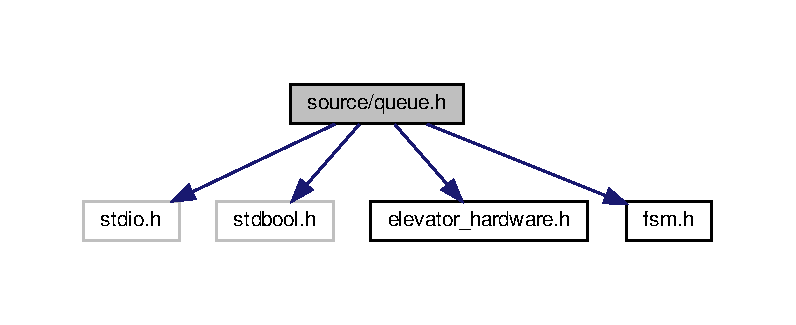
\includegraphics[width=350pt]{queue_8h__incl}
\end{center}
\end{figure}
This graph shows which files directly or indirectly include this file\+:\nopagebreak
\begin{figure}[H]
\begin{center}
\leavevmode
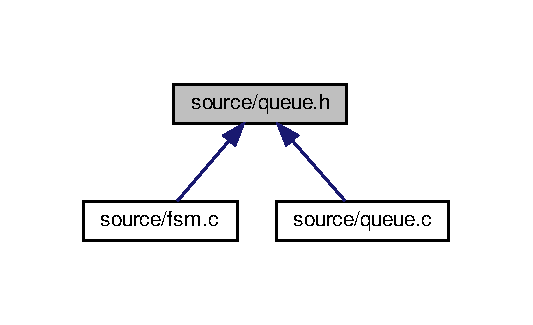
\includegraphics[width=256pt]{queue_8h__dep__incl}
\end{center}
\end{figure}
\subsection*{Functions}
\begin{DoxyCompactItemize}
\item 
void \hyperlink{queue_8h_a600fb7cf1ff3b028fcb97aa1af196065}{queue\+\_\+reset\+\_\+queue} ()
\begin{DoxyCompactList}\small\item\em Deletes all orders in the queue by setting all the order options to the initial value 0. \end{DoxyCompactList}\item 
void \hyperlink{queue_8h_a6b21f1da6ba83e1ee8ac5a64854415b7}{queue\+\_\+delete\+\_\+order} (\hyperlink{fsm_8h_a5b3a976f46b9e6993f1692a09bf2fd60}{floor\+\_\+t} floor)
\begin{DoxyCompactList}\small\item\em Deletes an order in the queue. \end{DoxyCompactList}\item 
void \hyperlink{queue_8h_ad9bbc447a9b368307ff0ea803d6c0fe1}{queue\+\_\+set\+\_\+order} (\hyperlink{elevator__hardware_8h_a5457414cc26332731098d18c37a46e6c}{elev\+\_\+button\+\_\+type\+\_\+t} button, \hyperlink{fsm_8h_a5b3a976f46b9e6993f1692a09bf2fd60}{floor\+\_\+t} floor)
\begin{DoxyCompactList}\small\item\em Sets an order in the queue. \end{DoxyCompactList}\item 
bool \hyperlink{queue_8h_a5f1a2d18955993f8c78589a8ce56dae9}{queue\+\_\+is\+\_\+queue\+\_\+empty} ()
\begin{DoxyCompactList}\small\item\em Checks whether the queue has any orders. \end{DoxyCompactList}\item 
\hyperlink{elevator__hardware_8h_ac873de158b370a210216e4b4c7fb218f}{elev\+\_\+motor\+\_\+direction\+\_\+t} \hyperlink{queue_8h_af2c4aec8d254eec04f73df6b5bba25d4}{queue\+\_\+get\+\_\+next\+\_\+direction} (\hyperlink{fsm_8h_a31f24aef3ddd32d2e6538ffff4055d37}{position\+\_\+t} current\+\_\+position, \hyperlink{elevator__hardware_8h_ac873de158b370a210216e4b4c7fb218f}{elev\+\_\+motor\+\_\+direction\+\_\+t} last\+\_\+direction)
\begin{DoxyCompactList}\small\item\em Checks if the elevator has any orders above, below or at its current position. The function will choose the next direction of the elevator based on these values and will prioritize the orders that is in the direction of the elevator. \end{DoxyCompactList}\item 
bool \hyperlink{queue_8h_a83fd2eb719d7deb1b38cbe8e00603eea}{queue\+\_\+should\+\_\+stop} (\hyperlink{fsm_8h_a31f24aef3ddd32d2e6538ffff4055d37}{position\+\_\+t} \hyperlink{fsm_8c_a740b52d852a7ed32ae50f2433e7fc8dd}{fsm\+\_\+position}, \hyperlink{fsm_8h_a5b3a976f46b9e6993f1692a09bf2fd60}{floor\+\_\+t} \hyperlink{fsm_8c_ae58b9d6bb7b780f3c1e7fd26baeb5683}{fsm\+\_\+floor}, \hyperlink{elevator__hardware_8h_ac873de158b370a210216e4b4c7fb218f}{elev\+\_\+motor\+\_\+direction\+\_\+t} \hyperlink{fsm_8c_a34c0ceaa7f628cf25af6d97bb6775eb4}{fsm\+\_\+direction})
\begin{DoxyCompactList}\small\item\em Checks if the elevator should stop when arriving at a floor, based on orders in the queue array. This function will inform the elevator that it should stop if\+: \end{DoxyCompactList}\end{DoxyCompactItemize}


\subsection{Detailed Description}
A queue system that helps the finite state machine (fsm) to carry out the orders received from the elevator hardware. 



\subsection{Function Documentation}
\mbox{\Hypertarget{queue_8h_a6b21f1da6ba83e1ee8ac5a64854415b7}\label{queue_8h_a6b21f1da6ba83e1ee8ac5a64854415b7}} 
\index{queue.\+h@{queue.\+h}!queue\+\_\+delete\+\_\+order@{queue\+\_\+delete\+\_\+order}}
\index{queue\+\_\+delete\+\_\+order@{queue\+\_\+delete\+\_\+order}!queue.\+h@{queue.\+h}}
\subsubsection{\texorpdfstring{queue\+\_\+delete\+\_\+order()}{queue\_delete\_order()}}
{\footnotesize\ttfamily void queue\+\_\+delete\+\_\+order (\begin{DoxyParamCaption}\item[{\hyperlink{fsm_8h_a5b3a976f46b9e6993f1692a09bf2fd60}{floor\+\_\+t}}]{floor }\end{DoxyParamCaption})}



Deletes an order in the queue. 


\begin{DoxyParams}[1]{Parameters}
\mbox{\tt in}  & {\em floor} & Floor the elevator is at \\
\hline
\mbox{\tt out}  & {\em queue\+\_\+array} & Queue table \\
\hline
\end{DoxyParams}


Definition at line 35 of file queue.\+c.

Here is the call graph for this function\+:\nopagebreak
\begin{figure}[H]
\begin{center}
\leavevmode
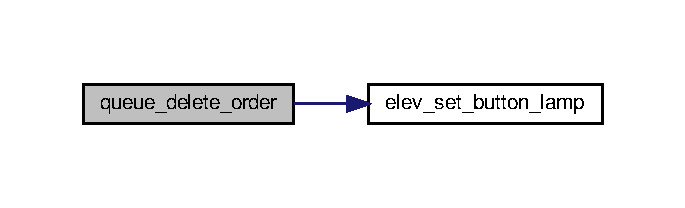
\includegraphics[width=329pt]{queue_8h_a6b21f1da6ba83e1ee8ac5a64854415b7_cgraph}
\end{center}
\end{figure}
\mbox{\Hypertarget{queue_8h_af2c4aec8d254eec04f73df6b5bba25d4}\label{queue_8h_af2c4aec8d254eec04f73df6b5bba25d4}} 
\index{queue.\+h@{queue.\+h}!queue\+\_\+get\+\_\+next\+\_\+direction@{queue\+\_\+get\+\_\+next\+\_\+direction}}
\index{queue\+\_\+get\+\_\+next\+\_\+direction@{queue\+\_\+get\+\_\+next\+\_\+direction}!queue.\+h@{queue.\+h}}
\subsubsection{\texorpdfstring{queue\+\_\+get\+\_\+next\+\_\+direction()}{queue\_get\_next\_direction()}}
{\footnotesize\ttfamily \hyperlink{elevator__hardware_8h_ac873de158b370a210216e4b4c7fb218f}{elev\+\_\+motor\+\_\+direction\+\_\+t} queue\+\_\+get\+\_\+next\+\_\+direction (\begin{DoxyParamCaption}\item[{\hyperlink{fsm_8h_a31f24aef3ddd32d2e6538ffff4055d37}{position\+\_\+t}}]{current\+\_\+position,  }\item[{\hyperlink{elevator__hardware_8h_ac873de158b370a210216e4b4c7fb218f}{elev\+\_\+motor\+\_\+direction\+\_\+t}}]{last\+\_\+direction }\end{DoxyParamCaption})}



Checks if the elevator has any orders above, below or at its current position. The function will choose the next direction of the elevator based on these values and will prioritize the orders that is in the direction of the elevator. 


\begin{DoxyParams}[1]{Parameters}
\mbox{\tt in}  & {\em current\+\_\+position} & The current position of the elevator \\
\hline
\mbox{\tt in}  & {\em last\+\_\+direction} & The direction of travel of the elevator.\\
\hline
\end{DoxyParams}
\begin{DoxyReturn}{Returns}
next direction of the elevator. 
\end{DoxyReturn}


Definition at line 64 of file queue.\+c.

Here is the caller graph for this function\+:\nopagebreak
\begin{figure}[H]
\begin{center}
\leavevmode
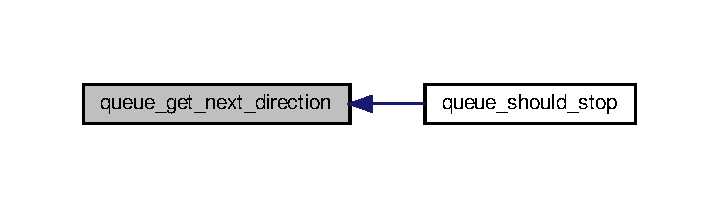
\includegraphics[width=345pt]{queue_8h_af2c4aec8d254eec04f73df6b5bba25d4_icgraph}
\end{center}
\end{figure}
\mbox{\Hypertarget{queue_8h_a5f1a2d18955993f8c78589a8ce56dae9}\label{queue_8h_a5f1a2d18955993f8c78589a8ce56dae9}} 
\index{queue.\+h@{queue.\+h}!queue\+\_\+is\+\_\+queue\+\_\+empty@{queue\+\_\+is\+\_\+queue\+\_\+empty}}
\index{queue\+\_\+is\+\_\+queue\+\_\+empty@{queue\+\_\+is\+\_\+queue\+\_\+empty}!queue.\+h@{queue.\+h}}
\subsubsection{\texorpdfstring{queue\+\_\+is\+\_\+queue\+\_\+empty()}{queue\_is\_queue\_empty()}}
{\footnotesize\ttfamily bool queue\+\_\+is\+\_\+queue\+\_\+empty (\begin{DoxyParamCaption}{ }\end{DoxyParamCaption})}



Checks whether the queue has any orders. 

\begin{DoxyReturn}{Returns}
1 if the queue is empty, 0 if not. 
\end{DoxyReturn}


Definition at line 48 of file queue.\+c.

\mbox{\Hypertarget{queue_8h_a600fb7cf1ff3b028fcb97aa1af196065}\label{queue_8h_a600fb7cf1ff3b028fcb97aa1af196065}} 
\index{queue.\+h@{queue.\+h}!queue\+\_\+reset\+\_\+queue@{queue\+\_\+reset\+\_\+queue}}
\index{queue\+\_\+reset\+\_\+queue@{queue\+\_\+reset\+\_\+queue}!queue.\+h@{queue.\+h}}
\subsubsection{\texorpdfstring{queue\+\_\+reset\+\_\+queue()}{queue\_reset\_queue()}}
{\footnotesize\ttfamily void queue\+\_\+reset\+\_\+queue (\begin{DoxyParamCaption}{ }\end{DoxyParamCaption})}



Deletes all orders in the queue by setting all the order options to the initial value 0. 


\begin{DoxyParams}[1]{Parameters}
\mbox{\tt out}  & {\em queue\+\_\+array} & Queue table \\
\hline
\end{DoxyParams}


Definition at line 24 of file queue.\+c.

Here is the call graph for this function\+:\nopagebreak
\begin{figure}[H]
\begin{center}
\leavevmode
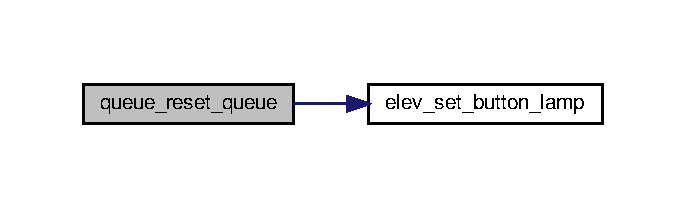
\includegraphics[width=329pt]{queue_8h_a600fb7cf1ff3b028fcb97aa1af196065_cgraph}
\end{center}
\end{figure}
\mbox{\Hypertarget{queue_8h_ad9bbc447a9b368307ff0ea803d6c0fe1}\label{queue_8h_ad9bbc447a9b368307ff0ea803d6c0fe1}} 
\index{queue.\+h@{queue.\+h}!queue\+\_\+set\+\_\+order@{queue\+\_\+set\+\_\+order}}
\index{queue\+\_\+set\+\_\+order@{queue\+\_\+set\+\_\+order}!queue.\+h@{queue.\+h}}
\subsubsection{\texorpdfstring{queue\+\_\+set\+\_\+order()}{queue\_set\_order()}}
{\footnotesize\ttfamily void queue\+\_\+set\+\_\+order (\begin{DoxyParamCaption}\item[{\hyperlink{elevator__hardware_8h_a5457414cc26332731098d18c37a46e6c}{elev\+\_\+button\+\_\+type\+\_\+t}}]{button,  }\item[{\hyperlink{fsm_8h_a5b3a976f46b9e6993f1692a09bf2fd60}{floor\+\_\+t}}]{floor }\end{DoxyParamCaption})}



Sets an order in the queue. 


\begin{DoxyParams}[1]{Parameters}
\mbox{\tt in}  & {\em button} & Hardware buttons \\
\hline
\mbox{\tt in}  & {\em floor} & At a floor \\
\hline
\mbox{\tt out}  & {\em queue\+\_\+array} & Queue table \\
\hline
\end{DoxyParams}


Definition at line 43 of file queue.\+c.

\mbox{\Hypertarget{queue_8h_a83fd2eb719d7deb1b38cbe8e00603eea}\label{queue_8h_a83fd2eb719d7deb1b38cbe8e00603eea}} 
\index{queue.\+h@{queue.\+h}!queue\+\_\+should\+\_\+stop@{queue\+\_\+should\+\_\+stop}}
\index{queue\+\_\+should\+\_\+stop@{queue\+\_\+should\+\_\+stop}!queue.\+h@{queue.\+h}}
\subsubsection{\texorpdfstring{queue\+\_\+should\+\_\+stop()}{queue\_should\_stop()}}
{\footnotesize\ttfamily bool queue\+\_\+should\+\_\+stop (\begin{DoxyParamCaption}\item[{\hyperlink{fsm_8h_a31f24aef3ddd32d2e6538ffff4055d37}{position\+\_\+t}}]{fsm\+\_\+position,  }\item[{\hyperlink{fsm_8h_a5b3a976f46b9e6993f1692a09bf2fd60}{floor\+\_\+t}}]{fsm\+\_\+floor,  }\item[{\hyperlink{elevator__hardware_8h_ac873de158b370a210216e4b4c7fb218f}{elev\+\_\+motor\+\_\+direction\+\_\+t}}]{fsm\+\_\+direction }\end{DoxyParamCaption})}



Checks if the elevator should stop when arriving at a floor, based on orders in the queue array. This function will inform the elevator that it should stop if\+: 


\begin{DoxyItemize}
\item There are no further orders in the direction.
\item There are cab or hall calls in the direction of travel.
\end{DoxyItemize}


\begin{DoxyParams}[1]{Parameters}
\mbox{\tt in}  & {\em fsm\+\_\+position} & The current position of the elevator. \\
\hline
\mbox{\tt in}  & {\em fsm\+\_\+floor} & The current floor of the elevator. \\
\hline
\mbox{\tt in}  & {\em fsm\+\_\+direction} & The direction of travel the elevator.\\
\hline
\end{DoxyParams}
\begin{DoxyReturn}{Returns}
1 of the elevator should stop, 0 if not. 
\end{DoxyReturn}


Definition at line 88 of file queue.\+c.

Here is the call graph for this function\+:\nopagebreak
\begin{figure}[H]
\begin{center}
\leavevmode
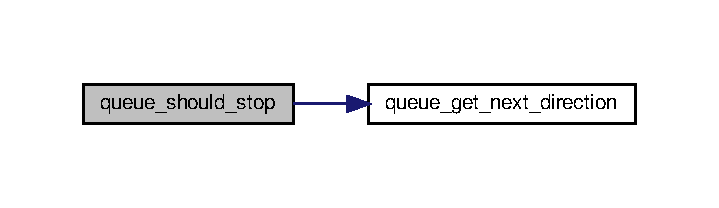
\includegraphics[width=345pt]{queue_8h_a83fd2eb719d7deb1b38cbe8e00603eea_cgraph}
\end{center}
\end{figure}

\hypertarget{timer_8h}{}\section{source/timer.h File Reference}
\label{timer_8h}\index{source/timer.\+h@{source/timer.\+h}}


A smaller module that manages the time dependent operations of the state machine.  


{\ttfamily \#include $<$stdio.\+h$>$}\newline
{\ttfamily \#include $<$stdbool.\+h$>$}\newline
{\ttfamily \#include $<$time.\+h$>$}\newline
Include dependency graph for timer.\+h\+:\nopagebreak
\begin{figure}[H]
\begin{center}
\leavevmode
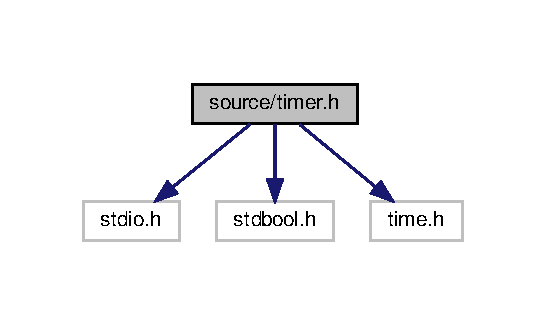
\includegraphics[width=262pt]{timer_8h__incl}
\end{center}
\end{figure}
This graph shows which files directly or indirectly include this file\+:\nopagebreak
\begin{figure}[H]
\begin{center}
\leavevmode
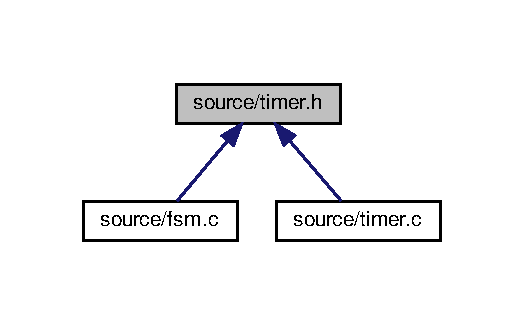
\includegraphics[width=252pt]{timer_8h__dep__incl}
\end{center}
\end{figure}
\subsection*{Functions}
\begin{DoxyCompactItemize}
\item 
time\+\_\+t \hyperlink{timer_8h_a4f7af40cfc5b42ea4f3ecd8e733a5bbf}{timer\+\_\+start\+\_\+timer} ()
\begin{DoxyCompactList}\small\item\em Starts a fictious timer by returning timestamp of the current time of the system. \end{DoxyCompactList}\item 
bool \hyperlink{timer_8h_a01822a31178b24ba570dd599a4549432}{timer\+\_\+is\+\_\+timer\+\_\+expired} (time\+\_\+t start\+\_\+timestamp)
\begin{DoxyCompactList}\small\item\em Check whether 3 seconds have passed since the timer started. \end{DoxyCompactList}\end{DoxyCompactItemize}


\subsection{Detailed Description}
A smaller module that manages the time dependent operations of the state machine. 



\subsection{Function Documentation}
\mbox{\Hypertarget{timer_8h_a01822a31178b24ba570dd599a4549432}\label{timer_8h_a01822a31178b24ba570dd599a4549432}} 
\index{timer.\+h@{timer.\+h}!timer\+\_\+is\+\_\+timer\+\_\+expired@{timer\+\_\+is\+\_\+timer\+\_\+expired}}
\index{timer\+\_\+is\+\_\+timer\+\_\+expired@{timer\+\_\+is\+\_\+timer\+\_\+expired}!timer.\+h@{timer.\+h}}
\subsubsection{\texorpdfstring{timer\+\_\+is\+\_\+timer\+\_\+expired()}{timer\_is\_timer\_expired()}}
{\footnotesize\ttfamily bool timer\+\_\+is\+\_\+timer\+\_\+expired (\begin{DoxyParamCaption}\item[{time\+\_\+t}]{start\+\_\+timestamp }\end{DoxyParamCaption})}



Check whether 3 seconds have passed since the timer started. 


\begin{DoxyParams}[1]{Parameters}
\mbox{\tt in}  & {\em start\+\_\+time} & Start time of timer.\\
\hline
\end{DoxyParams}
\begin{DoxyReturn}{Returns}
1 if the timer is expired, 0 if not. 
\end{DoxyReturn}


Definition at line 17 of file timer.\+c.

\mbox{\Hypertarget{timer_8h_a4f7af40cfc5b42ea4f3ecd8e733a5bbf}\label{timer_8h_a4f7af40cfc5b42ea4f3ecd8e733a5bbf}} 
\index{timer.\+h@{timer.\+h}!timer\+\_\+start\+\_\+timer@{timer\+\_\+start\+\_\+timer}}
\index{timer\+\_\+start\+\_\+timer@{timer\+\_\+start\+\_\+timer}!timer.\+h@{timer.\+h}}
\subsubsection{\texorpdfstring{timer\+\_\+start\+\_\+timer()}{timer\_start\_timer()}}
{\footnotesize\ttfamily time\+\_\+t timer\+\_\+start\+\_\+timer (\begin{DoxyParamCaption}{ }\end{DoxyParamCaption})}



Starts a fictious timer by returning timestamp of the current time of the system. 

\begin{DoxyReturn}{Returns}
the start time. 
\end{DoxyReturn}


Definition at line 12 of file timer.\+c.


%--- End generated contents ---

% Index
\backmatter
\newpage
\phantomsection
\clearemptydoublepage
\addcontentsline{toc}{chapter}{Index}
\printindex

\end{document}
